\chapter{Análise Bibliográfica sobre a Digitalização no Meio Educacional por Marcus Abrantes \label{chap:bibliometria:MarcusABR}}

\section{Planejamento do estudo}

A digitalização crescente tem transformado o comércio de informações. Quando bem empregada, possui o potencial de corrigir desigualdades, aperfeiçoar métodos e quebrar barreiras físicas. Este trabalho tem como objetivo analisar as últimas pesquisas a conclusões acerca das melhorias que a digitalização trouxe a meio educacional, bem como novas técnicas de ensino, dando atenção especial a gameficação. Uma técnica especial que surge inspirada em jogos para capturar a atenção dos estudantes e manter seu engajamento.

As seguintes pergunta foram usadas para nortear a pesquisa:
 

\begin{itemize}
    \item Qual a relevância e a atenção dada a pesquisa do uso de tecnologia na educação nos últimos anos?
    \item A gameficação tem sido considerada como uma técnica pertinente na avaliação de métodos de ensino.
    \item Nos últimos anos com o evento da pandemia, este assunto tem alçado maior importância, dados os desafios apresentados?
\end{itemize}

\subsection{Limitações} O trabalho foi desenvolvido ao decorrer de uma semana, empregando por volta de 5 a 10 horas.

\section{Coleta de dados}

A coleta de dados feita usando o mecanismo Web of Science no dia 09 de fevereiro de 2022, acessado por meio do Portal de Periódicos da CAPES.

\subsection{Query de Busca}

Para a busca dos artigo, foi usada a seguinte query:
\begin{verbatim}
educ*
and
(digital*  or gamific*)
and
improv*
and
learn*
\end{verbatim}

\subsubsection{Explicação para os termos de busca usados\label{}}

Tendo como tópico central a educação o termo \texttt{educ*}  foi utilizado. Com enfoque no meio digital, usa-se o termo \texttt{digita*} e para aumentar a abragência para  a técnica de gameficação, o termo \texttt{or} \texttt{gamefic*}. Como este trabalho tem enfoque nas melhorias trazidas pelo meio digital, e não nas consequências e desafios de seu uso, os termos \texttt{improv*}. Ainda, para reduzir a generalidade e tratar mais das vantagens no contexto de aprendisado, também foi o usado o termo \texttt{learn*}


\subsection{Registros recuperados}

 Os 7795 registros obtidos na busca podem ser encontrados no link ...
Foi utilizado o recurso \textit{Exportar registros para arquivo de texto sem formatação}, com todos as 29 opções de campo disponíveis. Os 7795 registros foram recuperado em grupos de 1000 para posteriormente serem concatenados.

\section{Análise dos dados}

\subsection{Filtragem de registros}


O registo inicial do \dataset\ possui 7795, para reduzir seu número e efetuar a a análise apenas sobre os documentos mais pertinentes, foram aplicados filtros. Primeiramente, foram excluídos todos os registros não caracterizados como artigos publicados em revistas científicas. Após isso, usando a lei de Bradford, os documentos foram reduzidos para apenas as fontes principais. Após a filtragem 1124 arquivos foram selecionados.

\subsection{Análise descritiva do \dataset\   }

Constam as informações gerais sobre os conjuntos de dados:
\begin{description}
    \item [\textit{Timespan}] Os artgiso obtidos da busca após a filtragem foram publicados entre o período de 1991 até 2022.
    \item [\textit{Sources (Journals, Books, etc)}] Os artigos possuem ao todo 29 fontes diferentes, sendo assim, em média, 39 artigos por revista.
    \item [\textit{Average years from publication}] A média de tempo de publicação dos artigos é de 4.26 anos.
    \item [\textit{Average citations per documents}] A média de citações por documentos é 18,35..
    \item [\textit{Average citations per year per doc}] Após o ano de sua publicação, das um dos dos artigos foi citado em média 2713 vezes por ano.
    \item [\textit{References}] Ao todo, foram feitas 46553  referências por entre os artigos coletados.
    \item [\textit{Keywords Plus (ID)}] 1828 palavras chaves do tipo ID (Keyword Plus).
    \item [\textit{Author's Keywords (DE)}]  3211 palavras chaves escolhidas pelos autores dos artigos.

    \item [\textit{Authors}]  Ao todo, foram encontrados 3874 autores no dataset.
    \item [\textit{Author Appearances}]  Os 3874 nomes apareceram 4543 vezes nos documentos.
    \item [\textit{Authors of single-authored documents}] Dos 3874 autoes, 81 escreveram artigos individualmente
    \item [\textit{Authors of multi-authored documents}] Dos 3874 autores, 3793 são autores de artigos escritos em colaboração com outros.
    \item [\textit{Single-authored documents}] Dos 1124 documentos, 85 foram escritos indidualmente, os 1039 restantes foram produzidos em co-autoria.
    \item [\textit{Documents per Author}] A média de documentos por autor é de 0.29.
    \item [\textit{Authors per Document}] A média de autores por dcumento é de 3.45.
    \item [\textit{Co-Authors per Documents}] As 4543 aparições de autores se distribuem em 4.04 por documento.
    \item [\textit{Collaboration Index}] O indíce de colaboração (total de autores em artigos escritos em co-autoria / total de artigos escritos em co-autoria) é de 3,65.
\end{description}

\subsection{Evolução da Produção Científica}



\begin{figure}[ht]
    \centering
    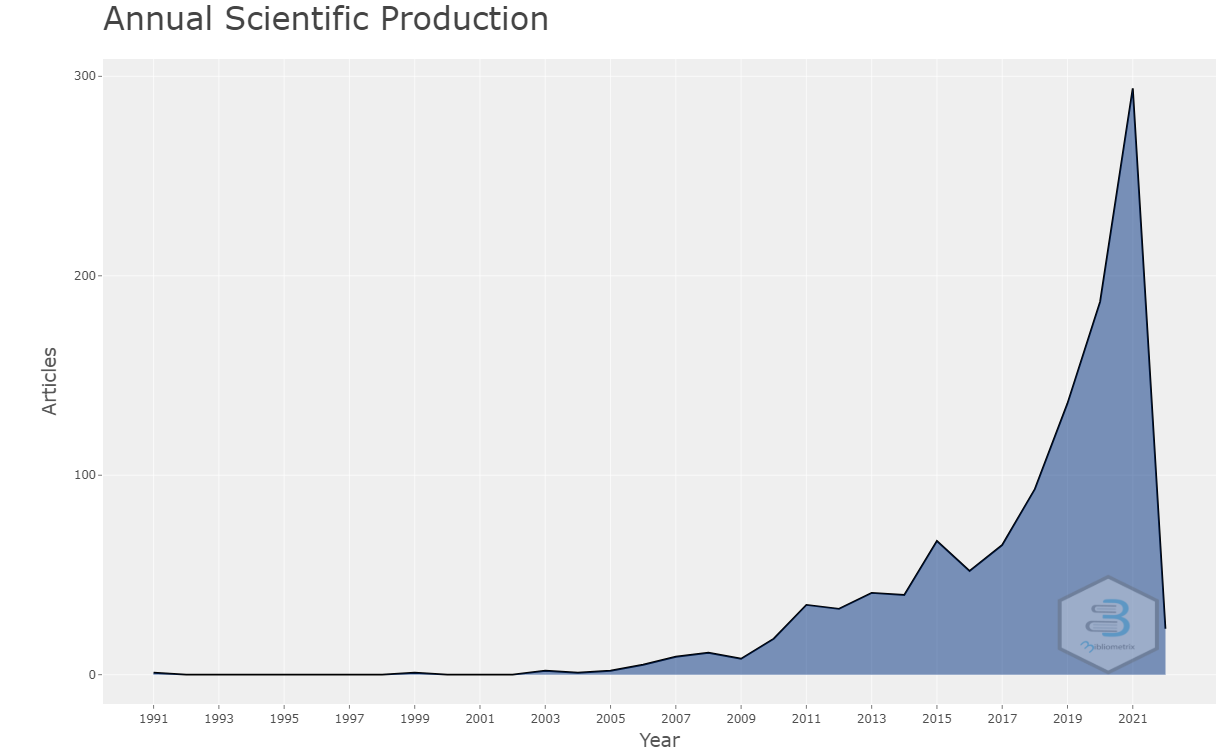
\includegraphics[width=12cm]{experiments/MarcusABR/PesquisaBibliometrica/Imagens/newplot.png}
    \caption{Evolução da produção científica no \dataset\ }
    \label{fig:evolucao}
\end{figure}

Conforme demonstra o gráfico houve uma crescente, alcançando o seu age dura os anos da pandemia entre 2019-2021

Nos anos de 2019-2021, em particular, foram introduzidas novas placas de vídeo no mercado, com poder computacional bem maior que as anteriores (é possível comparar as placas 1080 com as gerações 2080 e 3080 e perceber um aumento substancial de qualidade).

\subsection{Evolução das Citações}

A figura em \ref{fig:} mostra o número de citações médias feitas por ano. Nota-se uma grande quantidade de citações no ano de 2007, provavelmente devido a um artigo muito citado por outros autores. Nota-se também o que em uma faixa de 40 anos (1981-2021) o número de citações por ano aumentou de 0.2 para 1.0, um aumento de 5 vezes.

\begin{figure}[ht]
    \centering
    \includegraphics[width=12cm]{experiments/MarcusABR/PesquisaBibliometrica/Imagens/network(1).png}
    \caption{Evolução das citações por ano no \textit{}}
    \label{fig:gpu-citation-year}
\end{figure}

\subsection{\textit{Gráfico de três campos}}

O gráfico em \ref{fig:} mostra um gráfico de três campos feitos com os dados acerca das referências, autores e palavras-chaves mais relevantes.

\begin{figure}[ht]
    \centering
    \includegraphics[width=12cm]{experiments/MarcusABR/PesquisaBibliometrica/Imagens/network(3).png}
    \caption{Gráfico de três campos analisando palavras-chave no \textit{db\_GPU}}
    \label{fig:gpu-three-field}
\end{figure}

Observando as palavras-chaves, é possível perceber que termos como iluminação, processamento em paralelo e \textit{ray tracing} são expressões relevantes no contexto de GPUs.

Em particular, a técnica de \textit{Ray Tracing} foi otimizada nos últimos anos, de forma que é possível aplicá-la em simulações em tempo real (que antes não era possível devido ao alto custo computacional).

Observando os autores é possível perceber que a maior parte é de origem asiática e que esses autores utilizam principalmente \textit{masuda n 2006 opt express} como referência.

Essa publicação em específico relata avanços feitos na redução do custo computacional para geração de hologramas (objetos tridimensionais) em ambientes computacionais.

\subsection{Refinamento da coleta de dados}

O gráfico em \ref{fig:gpu-co-occur} mostra a rede de co-ocorrências de palavras-chave no \textit{db\_GPU}. Dentro os termos é possível perceber que os assuntos tratados são relevantes ao tópico de GPUs, com destaque ao campo em verde que separa assuntos relativos a dispersão de luz em meios turbulentos (\textit{turbid media}).

\begin{figure}[ht]
    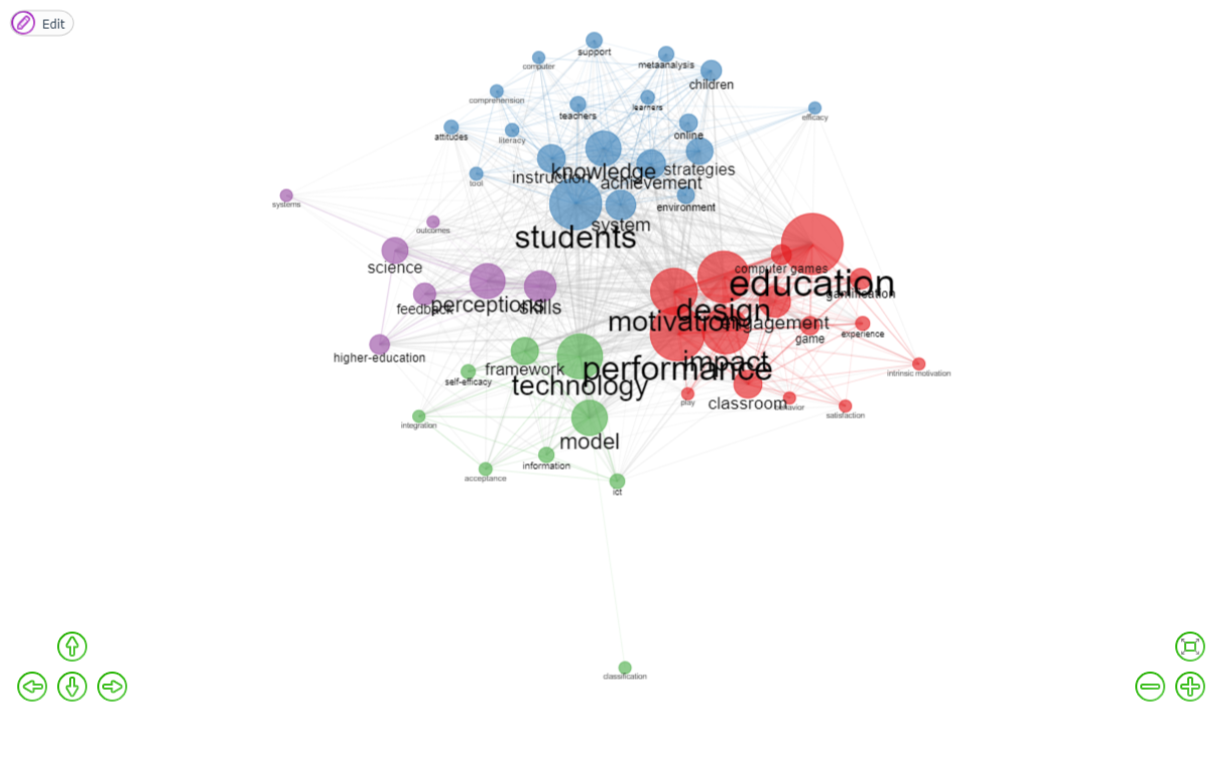
\includegraphics[width=12cm]{experiments/MarcusABR/PesquisaBibliometrica/Imagens/network.png}
    \caption{Rede de co-ocorrências de palavras-chave no \textit{db\_GPU}}
    \label{fig:gpu-co-occur}
\end{figure}

Esses tópicos são de especial interesse ao tópico de simulação de luz, pois essa simulação se dá por meio de aproximações ao mundo real (modelos físicos e fórmulas matemáticas). Um modelo eficiente consegue reter a essência dos fenômenos reais, de modo que é possível realizar uma simulação realista com uma capacidade computacional não tão elevada.

Softwares de animação (como blender) e de simulação possuem \textit{engines} que simulam fenômenos físicos, tais como corpos sólidos, emissores, índice de refração de materiais e reflexo da luz. Em especial, a \textbf{simulação de Monte Carlo} permite que uma amostra aleatória de possíveis caminhos de luz convirjam para uma solução correta, tornando esse método um dos métodos físicos mais precisos existentes.

